\documentclass[SoftwareDesign/SoftwareDesign_main.tex]{subfiles}

\begin{document}
\section{Side Navigation}
Før vi kommer mere ind på selve designet af de enkelte Views og Viewmodels, så er det en god ide og se på hvordan hele navigationssystemet er sat op. Det er nemlig vigtigt for CarnGo appen at der kan navigeres mellem de forskellige sider, når først brugeren er logget ind. Der vil efter login vises en startside, hvor brugeren herfra kan navigerer til forskellige sider ved hjælp af en headerbar, hvorefter det fra nogle af siderne også vil være muligt at navigere til andre sider igennem selve sidens design. \\
For at kunne implementere dette skulle en singleton bruges, der kunne tilgås fra alle siderne, så alle sider i teorien ville have mulighed for at skifte til de sider, den har brug for at skifte til. Det er essentielt, at det er samme instans de anvender. Hertil blev klassen ApplicationViewmodel lavet. 

Det essentielle ved dette navigationssystem, er at opretholde lav kobling mellem ViewModllerne og stadigvæk opretholde MVVM-principperne i forhold ingen direkte relation mellem Views og ViewModels. Hvis hvert ViewModel selv havde til ansvar for at skifte mellem Views, skulle de havde direkte adgang til hvert ViewModel. Dette vil desuden også medfører, at ViewModellerne skulle kende til tilhørende View, da de selv skulle stå for at initierere det. Begge ansvar er udliciteret til ApplicationViewModel. 

ApplicationViewmodel består af en usermodel(information om brugeren logget ind), funktioner til login af bruger, og en CurrentPage property, som holder en enum af typen ApplicationPage, der holder den nuværende side. Derudover er der en funktion(GoToPage) til at skifte CurrentPage Property. 

ApplicationViewModel er registreret som en singleton i en IOC-container, der er brugt i applikationen, og igennem denne kan siderne enten bruge containerens resolve funktion til at få fat i applicationViewModel eller IOC-container kan injecte den ind i sidernes ViewModels. 

Spørgsmålet er nu, hvordan der bliver skiftet imellem siderne bare ved at sætte CurrentPage Property i ApplicationViewModel. Dette er muligt, da der i MainWindowViewet er initialiseret en brugerdefineret usercontrol kaldet pagenavigation. Denne usercontrol har en dependencyproperty også kaldet CurrentPage af typen Page, som CurrentPage fra ApplicationViewModel databindes til. Da de to typer ikke er de samme, bruges en valueconverter til at konverterer fra typen ApplicationPage til Page. I det en ændring forekommer vil et event forekomme for CurrentPage dependencyproperty i PageNavigation og den nuværende frame(side) vil blive ændret. Nedenfor ses et klassediagram samt sekvensdiagram for dette. På klasse diagrammet i figur \ref{fig:PageNavigation_CD} ses alle klasserne involveret, når en side i applikationen. Her er kun 2 ViewModels vist, selvom alle viewmodels er med. Dette blev gjort for at holde diagrammet overskueligt. LoginViewModel er her vist som en af de viewmodels, hvor man gennem siden skifter til en specifik side. HeaderBarViewmodel er der hele tiden efter man er logget ind i applikationen og det er gennem den muligt at skifte mellem flere forskellige sider. På figur \ref{fig:PageNavigation_SD} ses et sekvensdiagram, som beskriver skiftet fra Login viewet til StartPage viewet. Dette gælder selvfølgelig også for de to viewmodel, der tilhører de to views.
 
\begin{figure}[H]
    \centering
    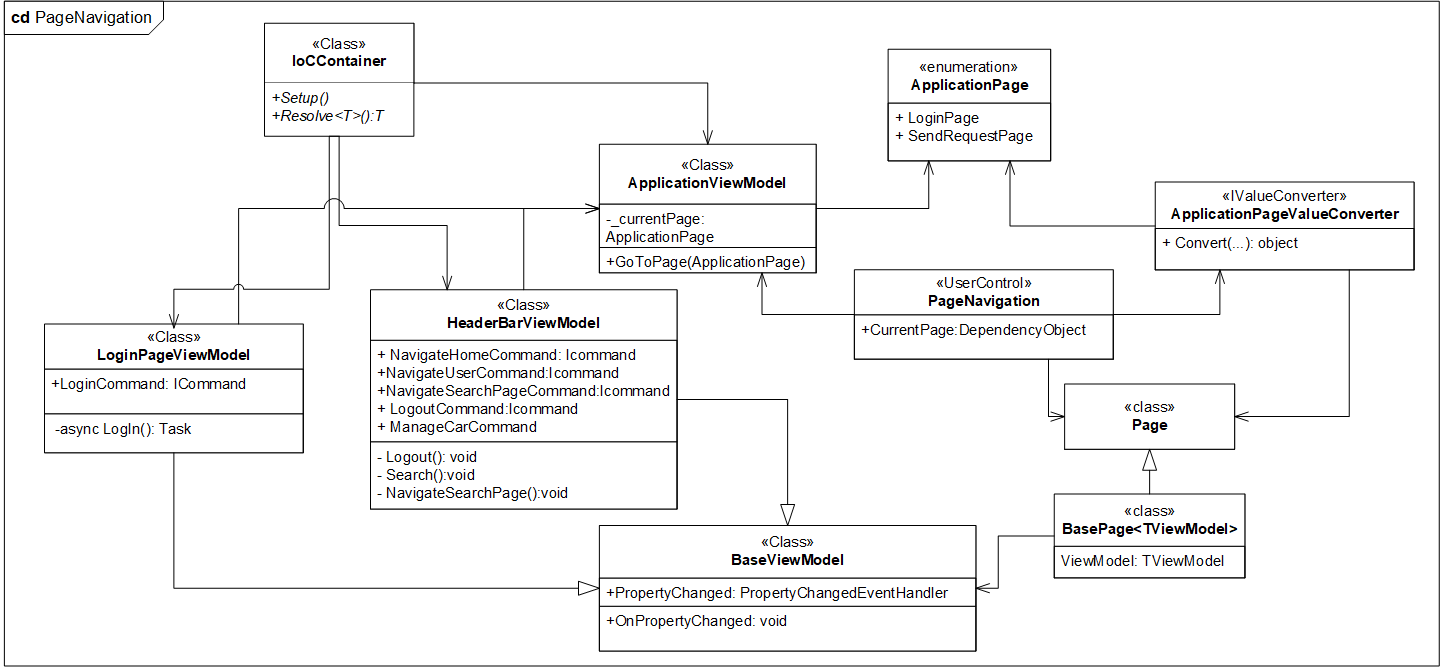
\includegraphics[width=\textwidth]{SoftwareDesign/MVVMDesigns/Graphics/PageNavigationcd.png}
    \caption{Her ses klassediagram for PageNavigation, hvor man ser de forskellige klasser involveret, når en side skal skiftes ud med en anden.}
    \label{fig:PageNavigation_CD}
\end{figure}
\begin{figure}[H]
    \centering
    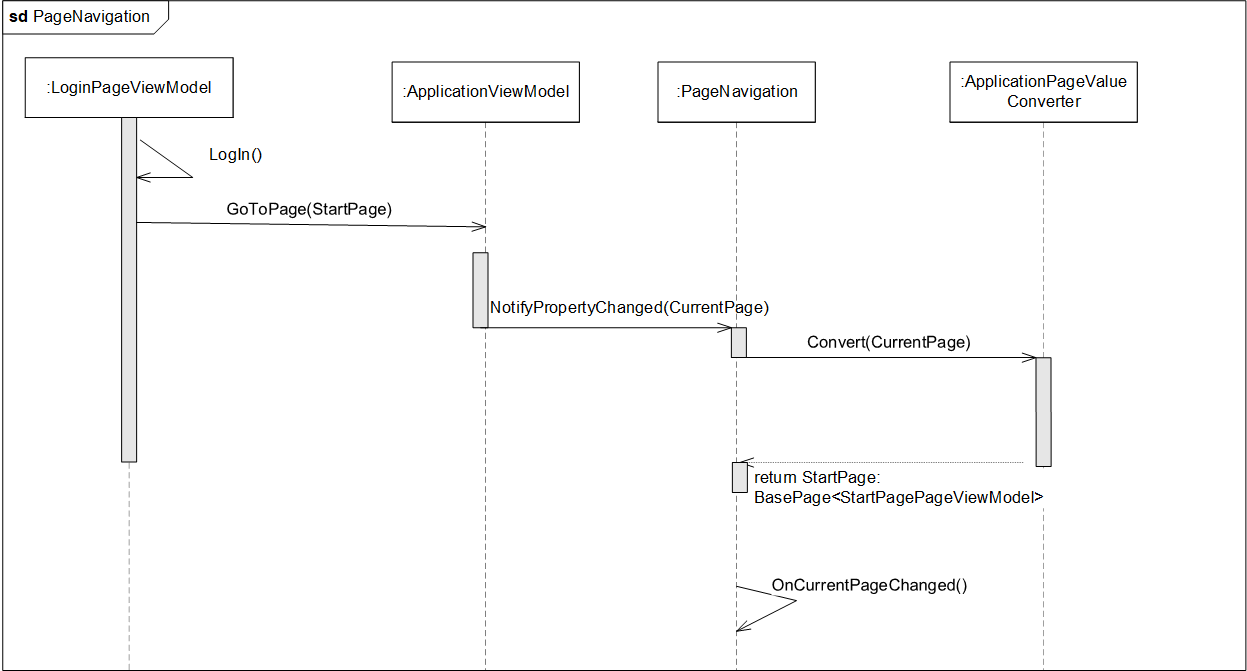
\includegraphics[width=\textwidth]{SoftwareDesign/MVVMDesigns/Graphics/PageNavigationSd.png}
    \caption{Her ses sekvensdiagrammet for PageNavigation, hvor Login skifter til StartPage Viewet}
    \label{fig:PageNavigation_SD}
\end{figure}

\end{document}